\documentclass[nobib]{tufte-handout}
\usepackage{graphicx} % Required for inserting images
\usepackage{float}

\title{Exercises}

\author[Group 2]{Arvid Stenarson, Koay Yong Sheng, Max Sundblad, Nils Eriksson, Saeid Taghizadeh Sabetghadam}%\thanks{\href{mailto:vilhelm.agdur@math.uu.se}{\nolinkurl{vilhelm.agdur@math.uu.se}}}}

\date{13 November 2023}


%\geometry{showframe} % display margins for debugging page layout

\usepackage{graphicx} % allow embedded images
  \setkeys{Gin}{width=\linewidth,totalheight=\textheight,keepaspectratio}
  \graphicspath{{graphics/}} % set of paths to search for images
\usepackage{amsmath}  % extended mathematics
\usepackage{booktabs} % book-quality tables
\usepackage{units}    % non-stacked fractions and better unit spacing
\usepackage{multicol} % multiple column layout facilities
\usepackage{lipsum}   % filler text
\usepackage{fancyvrb} % extended verbatim environments
  \fvset{fontsize=\normalsize}% default font size for fancy-verbatim environments

\usepackage{color,soul} % Highlights for text

% Standardize command font styles and environments
\newcommand{\doccmd}[1]{\texttt{\textbackslash#1}}% command name -- adds backslash automatically
\newcommand{\docopt}[1]{\ensuremath{\langle}\textrm{\textit{#1}}\ensuremath{\rangle}}% optional command argument
\newcommand{\docarg}[1]{\textrm{\textit{#1}}}% (required) command argument
\newcommand{\docenv}[1]{\textsf{#1}}% environment name
\newcommand{\docpkg}[1]{\texttt{#1}}% package name
\newcommand{\doccls}[1]{\texttt{#1}}% document class name
\newcommand{\docclsopt}[1]{\texttt{#1}}% document class option name
\newenvironment{docspec}{\begin{quote}\noindent}{\end{quote}}% command specification environment

\include{mathcommands.extratex}


\newcounter{counter}

\newcommand\bb[1]{\mathbb{#1}}
\newcommand\cl[1]{\mathcal{#1}}
\newcommand\allbold[1]{{\boldmath\textbf{#1}}}
\newcommand\linematrix[1]{\begin{pmatrix}#1\end{pmatrix}}
\newcommand\intt[4]{\int_{#1}^{#2} #3 \, d#4}
\newcommand{\intdiff}[3]{\left[ #1 \right]_{#2}^{#3}}
\newcommand{\eval}[2]{\left.#1 \, \right|_{#2}}
\newcommand{\limm}[2]{\lim_{#1} \left(#2\right)}
\newcommand{\veq}{\mathrel{\rotatebox{90}{$=$}}}
\newcommand{\vneq}{\mathrel{\rotatebox{90}{$\neq$}}}
\newcommand{\vecbold}[1]{\mathbf{#1}}
\newcommand{\derleib}[2]{\dfrac{d#1}{d#2}}
\newcommand\pder[3][]{\dfrac{\partial^{#1} #2}{\partial #3^{#1}}}
\newcommand{\derlagr}[3][x]{#2^{(#3)}(#1)}
\newcommand{\sidecomment}[1]{\qquad\qquad \bigpar{\text{#1}}}
\newcommand{\arrowexpl}[2]{\underset{\substack{\uparrow\\\mathrlap{\text{\hspace{-1em}#2}}}}
{#1}}
\newcommand{\bigpar}[1]{\left(#1\right)}
\newcommand{\bigbrack}[1]{\left[#1\right]}
\newcommand{\bigset}[3][1]{%
    \ifthenelse{1=#1}{%
        \left\{#2 \left| \, #3 \right.\right\}
    }{%
        \left\{#2\right\}
    }
}
\newcommand{\dett}[4]{%
    \left| \hspace{-1mm} %
        \begin{array}{cc}
             #1 & #3 \\
             #2 & #4
        \end{array}%
    \hspace{-1.2mm} \right|}
\newcommand\summ[4]{%
    \ifthenelse{1=#4}{%
        \sum_{#1}^{#2}{\bigpar{#3}}
    }{%
        \sum_{#1}^{#2}#3
    }
}

\newenvironment{done}[1]{\vspace{2mm} \begin{center} $\therefore$ #1}{\end{center} \hfill \square}
\newenvironment{tagenv}[1]{\tag{#1\thecounter} \stepcounter{counter}}{}
\newcommand{\tagg}[1]{\begin{tagenv}{#1}\end{tagenv}}


\begin{document}

\maketitle% this prints the handout title, author, and date

%\begin{abstract}
%\noindent
%Stuff
%\end{abstract}
\section{Exercises 1}
    Prove that T'' actually is a spanning tree. \\ 

    \textbf{Answer:} \\ 
    Let $H$ be the graph formed by adding an edge $e$ not in $T'$ to $T'$. Since a tree is an edge-minimal acyclical connected graph the only possible outcome of this (in order to not contradict edge-minimality) is that $H$ contains a cycle. We then form $T''$ by removing an edge $f$ from this cycle. Since all vertices of $H$ were connected to the vertices of the cycle and removing an edge from a cycle keeps it connected, we have that $T''$ is connected through the remaining vertices of the cycle. We also have that $E(T'') = E(T') = n - 1$, hence $T''$ is a tree containing all vertices of $G$ (we haven't removed any vertices from $T'$ in the construction of $T''$), i.e.\ a spanning tree.

\newpage

\section{Exercises 2}
  Prove that this really is a tree. You can equivalently think of it as the union of all shortest paths between the root v and some other vertex. (This tree is called a shortest-path tree.) \\
  
  \textbf{Answer:} \\ 
  Let $G = (V, E)$ be a positively weighted connected graph with $|V| = n$. Dijkstra's algorithm creates a parent function $p$ s.t.\ all vertices in the resulting graph except $r$ is assigned a neigbouring parent vertex, i.e.\ one could equivalently view it as every vertex except $r$ being assigned the edge from it to its assigned parent. Hence the algorithm adds one edge per vertex except $r$ (notice such an edge may not be the same throughout all of the algorithm), i.e.\ upon termination we have a subgraph of $G$, $G'$, s.t.\ $E(G') \leq n - 1$. Since the algorithm always adds an incident edge of a vertex in question such that the vertex becomes connected to a path to the root $r$ we have that all vertices of $G'$ are connected to $r$ and as such that all vertices are connected to each other, i.e.\ $G'$ is connected. But we also know that trees are edge-minimal connected graphs and that a graph is a tree iff it is connected and has $n - 1$ edges. Hence $E(G') \geq n - 1$, and as such $E(G') = n - 1$. Hence $G'$ is a connected $n$-vertex graph of $n - 1$ edges, i.e.\ $G'$ is a tree.
\newpage

\section{Exercises 3}
We have shown in an exercise during our previous exercise session that a weighted graph with all weights distinct has a unique minimum spanning tree. \\  

Is the stronger statement that in fact no two spanning trees have the same weight also true? \\

\textbf{Answer:} \\ 
No it is not true.

For a graph $G = (V,E,w)$, where all weights w are distinct, we have a tree $T$. If there is a way to modify $T$ into tree $T^\prime$, which has the same weight as that of $T$, then the statement is false. 

As a tree $T$ always has $(|V|-1)$ edges, every edge added must result in an edge removed and vice versa. And as all weights are distinct no single edge can be switched out in a way that results in a tree with the same weight. So, for weight to be conserved, at least two edges must be removed and switched out for other ones. The condition is that the increase in weight from one edge switch must be counteracted by a decrease in weight from another switch. So, as long as there are unused edges that can facilitate a switch like that, it is indeed possible, which makes the statement false. This is easily shown in a figure.

\begin{figure}
    \centering
    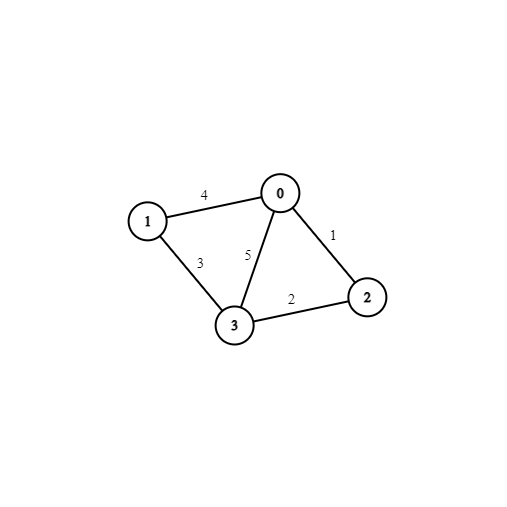
\includegraphics[width=0.5\textwidth]{graphics/L6_prim_kruskal_dijkstra/distinctWeights.png}
    \caption{Graph $G = (V,E,w)$}
    \label{fig:G}
\end{figure}

\begin{figure}
    \centering
    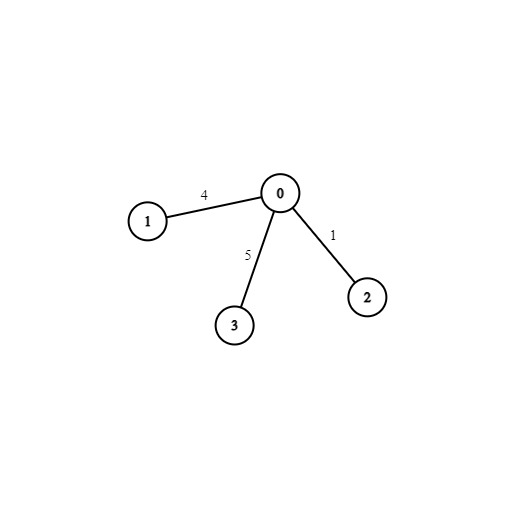
\includegraphics[width=0.5\textwidth]{graphics/L6_prim_kruskal_dijkstra/distinctWeights2.png}
    \caption{Tree $T$ with weight 10}
    \label{fig:T}
\end{figure}

\begin{figure}
    \centering
    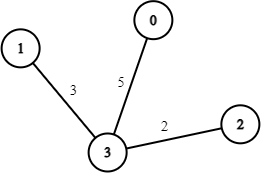
\includegraphics[width=0.5\textwidth]{graphics/L6_prim_kruskal_dijkstra/distinctWeights3.png}
    \caption{Tree $T^\prime$ with weight 10}
\end{figure}

As this can be done for at least some graphs, the statement is proven false.
\newpage

\section{Exercises 4}

  One way to find a path between two vertices is to first find a minimum spanning tree for the graph and then find the unique path between them in this tree.  

\textbf{Answer:} \\ 
\begin{enumerate}
    \item Will this always be the shortest path between them?
    
    No, there is no guarantee that this would be the shortest path between this two vertices. To show this, one can look at a specific example as a counterexample. Given a graph shown in the Figure\ref{fig:ex4_full} (left):
    \begin{itemize}
        \item it should be obvious for the reader that Figure\ref{fig:ex4_full} (middle) is an MST (If not, one can try to use Kruskal's or Dijkstra's algorithm to find it).
        \item Now, given the path to go from C to D via the path in the MST, one would lead to a path with total weight=7.
        \item However, in Figure\ref{fig:ex4_full} (right), we could have use a shorter path (with weight = 5) which the edge that was removed to form the MST.  
    \end{itemize}  
    
\begin{figure}
  \centering
  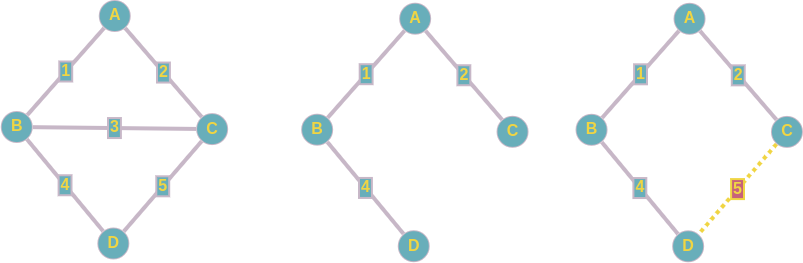
\includegraphics[width=0.85\textwidth]{graphics/L6_prim_kruskal_dijkstra/ex4_full.png}
  \caption[][0cm]{Left: Example weighted graph. Middle: MST. Right: Shorter Path from C to D}
  \label{fig:ex4_full}
\end{figure}

    \item If not, will there always be \emph{some} pair of vertices such that this is the shortest path between them?
    
    Yes, there will always be some pair of vertices such that this is the shortest path between them. This is true if edge(s), $e_{min}$ with minimum weight $w_{min}$ always exist in the MST. The shortest path between any two vertices that are connected by an $e_{min}$ should be the path with only $e_{min}$, (ie. P=$v_1e_{min}v_2$).\sidenote{Note that you can have more than one edge in a graph with the minimum weight. Also, one can have multiple shortest path between two vertices}.
    
    Since $e_{min}$ has minimum weight, any other shorter path between its vertices that is not this, would imply that either:
    \begin{itemize}
        \item there is an edge with a lower weight (which contradict with the definition of $e_{min}$) or
        \item there is a path that contains edges with negative weight (which contradict with the definition of distance, which is required to talk about \textit{"shortest"}) or
        \item another edge with minimum weight connected to the same pairs of vertices (which would just lead to another $e_{min}$ in another MST and also contradict the definition of a simple graph)
    \end{itemize}
    Now, one just need to prove that at least one $e_{min}$ would always exist in any MST, then we will have proved our statement. To do this, we will prove by contradiction.
    
    Given a graph, G(V,E) with $w(e_{min}) = w_{min}$ where $e_{min} =\{v_1,v_2\}$. We first consider the existence of $P=v_1 ... v_2$ where $w(P) = w$ and $w > w_{min}$: 
    \begin{enumerate}
        \item if P does not exist, then argument 1 already imply $e_{min}$ must be in the MST, since its the only way to connect $v_1 $ and $ v_2$.
        \item if P exist, then it implies the existence of a cycle in the graph since there are two ways of going from $v_1$ to $v_2$
    \end{enumerate}
    
    Now, in the scenario where P exist, assume that $e_{min}$ is not in the MST and P is. We can add $e_{min}$ into the MST to form a graph with cycle. Now if we remove the maximal edge in the cycle (this would not be $e_{min}$), this would again form a tree with the weight of the tree less than the weight of the MST, contradicting the definition of an MST. Hence, $e_{min}$ must always exist in an MST and thus, there will always be some pair of vertices such that the path in the MST is the shortest path between them.
    
\end{enumerate}
\newpage
\section{Exercise 5}

Are any of the things we did in this lecture useful for computing the diameter of a graph? Think about how one might do it, and what runtimes your suggested algorithms will have.

\textbf{Answers:}\\

It's pretty useful to know how to compute the distance between any two nodes in a weighted graph if you want to find the maximal distance. 

The most straightforward way to compute the diameter is just determining the distance function  \( d(v, \cdot), \forall v \in V \). This can be done via an algorithm which takes the current maximum distance  \( D \) as an argument . Start algorithm with \( D=0 \). Then for every vertex \( v\in V \), use Djikstras algorithm to find \( d(v,\cdot) \). If \( \max(d(v,\cdot))>D\), then set \(  D=\max(d(v,\cdot)) \). When you have iterated through all vertices, return \( D\). This will obviously give the diameter. Djikstras algorithm has runtime \( \mathcal{O}(|E|+|V| \log(|V|)) \). So this algorithm has runtime \( \mathcal{O}(|V|(|E|+|V| \log(|V|))) \). 

One could definitely utilise the fact that intialising Djikstras algorithm from a node, one also gets the distance between other nodes "for free". Not only is \( d(v,v')=d(v',v) \), but also the distances between any intermediate nodes are from \( v' \) to \( v \) is acquired. However, it seems somewhat complicated to determine a \( \Theta \) complexity for such an algorithm with our current knowledge. Probably, this task requires some knowledge about random trees. 

Searching the internet for a more effective algorithm I found the Floyd-Warshall algorithm which has a time complexity of \( \mathcal{O}(|V|^3) \). This algorithm uses a modified weighted adjacency matrix which finds the distance between all nodes simultaneously by considering each node as an intermediate node. For example, we might know that there is a path of length \( d\) from \( v \) to \( v' \), now consider if the path via \( v''\) is shorter: \( d(v,v'')+d(v'',v')<d(v,v') \)? The complexity of the Floyd-Warshall algorithm is preferred if the amount of edges greatly exceeds the amount of vertices, i.e. if the graph is dense. 

\newpage
\section{Exercise 6}
If there are multiple edges of the same weight there may be some indeterminacy in Prim's and Kruskal's algorithm. Show that all MST:s of a graph can be found using both of the algorithms.

\textbf{Answers:} \\ 
 \subsection{Kruskal's Reaches all MST:s}
            Let $T$ be an MST of $G = (V, E)$. \\
            
            Let $W$ be a $\leq$-ordered sequence of all the weights which appear in $G$. Then for $w \in W$ let $L_w^T$ be a sequence which orders the elements of $\bigset[1]{e \in E(T)}{w(e) = w}$, i.e.\ $L_w$ is an ordering of the edges in $T$ with weight $w$ (might be empty if there are no edges in $T$ of weight $w$), and Let $L_w^{\neg T}$ be a sequence which orders $\bigset[1]{e \in E \setminus E(T)}{w(e) = w}$. \\
            
            (Below we will use $\oplus$ for sequences and this will be interpreted as $(a_1, \ldots, a_m) \oplus (b_1, \ldots, b_n) = (a_1, \ldots, a_m, b_1, \ldots, b_n)$, and for an ordered sequence $I = (i_1, \ldots, i_k)$ we will interpret $\bigoplus\limits_{i \in I} A_i$ as $A_{i_1} \oplus \ldots \oplus A_{i_k}$) \\
            
            Now let $L_w = L_w^T \oplus L_w^{\neg T}$ and finally:
%
            \begin{align*}
                L = \bigoplus_{w \in W} L_w
            \end{align*}

            What we have constructed in the form of $L$ is a sequence of the edges in $E$ which is weight-ordered and for any weight $w \in W$ we have that all edges in $E(T)$ of weight $w$ appear first in the list followed by any residual edges in $E \setminus E(T)$ also of weight $w$. The list $L$ is what we will give Kruskal's algorithm as input and we now want to show that Kruskal's indeed returns $T$ upon termination. \\

            We will suppose for contradiction that there is some first timestep $i$ at which Kruskal's deviates from $T$. This deviation must be of the form that the algorithm adds an edge $e_i$ which is not in $T$. This is since the only other possible deviation would be that the algorithm does not add $e_i$ even though it is in $T$, but that would mean that adding $e_i$ creates a cycle with the already added edges all of which are in $T$ but this is not possible since that would mean there is a cycle in $T$. \\

            Now if we add $e_i$ to $T$ we create a cycle. This cycle must contain some edge of greater weight than $e_i$ since all edges in $T$ of weight $\leq w(e_i)$ have been added before $e_i$ by the algorithm ($e_i \in L_w(e_i)^{\neg T}$ which comes after $L_{w(e_i)}^T$ in $L$ and all the edges with weight strictly less than $w(e_i)$). Now if we remove this edge from the cycle we get a connected graph of $n - 1$ edges again, i.e.\ a spanning tree $T'$. We also have $w(T)' < w(T)$ which contradicts the fact that $T$ is an MST. Hence the algorithm does not deviate at any point, i.e.\ the algorithm produces $T$.

            
        
\subsection{Prims Algorithm Reaches all MST:s}

Let \(G={V,E} \) be a weighted graph with weight \( w \). Assume there is a MST \( T \) which Prims algorithm can't find. Define \( w' \) by removing a small amount \( \epsilon \) from the weight of each edge in T such that the \( 0<\epsilon<w(e_i)-w(e_j) \quad \forall e_i, e_j \in E: w(e_i)\neq w(e_j)\). This is now the unique MST of \(G \) with weights \( w' \). Prims algorithm can find this MST due to it being unique. In every step we are going to consider adding "valid" edges, we want to add the minimal "valid" edge so there is going to be ordering such that all \( w_i-\epsilon \) comes before all \( w_i\) but after \( w_j<w_i \) due to our choice of \( \epsilon \). But this means that the ordering is still proper with our original weight \( w \). So Prims algorithm can find \( T \quad \) %\scalebox{2}{\Lightning}

\end{document}
